\section{A new upper bound for the de Bruijn-Newman constant}\label{newup-sec}

In this section we prove Theorem \ref{new-upper}.  As stated in the introduction, it suffices to verify the conditions (i), (ii), (iii) of Theorem \ref{ubc-0} $t_0 \coloneqq 0.2$, $X \coloneqq X_0-0.5$, and $y_0 \coloneqq 0.2$, where $X_0 \coloneqq 6 \times 10^{10} + 83952$.  

Claim (i) is immediate from the result of Platt \cite{platt} that all the non-trivial zeroes of $\zeta$ with imaginary part between $0$ and $3.06 \times 10^{10}$ lie on the critical line $\{ \mathrm{Re}(s) = 1/2\}$.  For the remaining claims (ii), (iii), we need to verify that $H_t(x+iy) \neq 0$ for two regions of $(x,y,t)$:
\begin{itemize}
\item[(ii)]  $x \geq X_0 - 0.5 + \sqrt{0.96}$, $0.2 \leq y \leq \sqrt{0.6}$, and $t = 0.2$. 
\item[(iii)]  $X_0 - 0.5 \leq x \leq X_0 - 0.5 + \sqrt{0.96}$, $\sqrt{0.04 + 2(0.2-t)} \leq y \leq \sqrt{0.6}$, and $0 \leq t \leq 0.2$.
\end{itemize}
Both of these regions lie in \eqref{region}.  Enlarging the regions slightly, and applying Corollary \ref{zero-test}, it thus suffices to establish the following claim:

\begin{proposition}\label{sweep}  Let $(x,y,t)$ lie in one of the following regions:
\begin{itemize}
\item[(ii)] (Asymptotic zero free region) $x \geq X_0$, $0.2 \leq y \leq \sqrt{0.6}$, and $t = 0.2$.
\item[(iii)] (Barrier)  $X_0 - 0.5 \leq x \leq X_0 + 0.5$, $0.2 \leq y \leq \sqrt{0.6}$, and $0 \leq t \leq 0.2$.
\end{itemize}
Define
\begin{align*}
f_t(x+iy) &\coloneqq \sum_{n=1}^N \frac{b_n^t}{n^{s_*}} + \gamma \sum_{n=1}^N n^y \frac{b_n^t}{n^{\overline{s_*} + \kappa}}\\
b_n^t &\coloneqq \exp( \frac{t}{4} \log^2 n),\\
N &\coloneqq \lfloor \sqrt{\frac{x}{4\pi} + \frac{t}{16}} \rfloor \leq [\frac{x}{4\pi} (1 + \frac{\pi t}{4x})]^{1/2},
\end{align*}
so in particular
\begin{equation}\label{logx}
 \log \frac{x}{4\pi} \geq 2 \log N - \log(1 + \frac{\pi t}{4x}),
\end{equation}
and let $\kappa, s_*, \gamma, e_A, e_B, e_{C_0}$ be as in Theorem \ref{eff}, and $e_A, e_B, e_{C_0}$.  Then
\begin{equation}\label{bbb}
|f_t(x+iy)| > e_A + e_B + e_{C,0} 
\end{equation}
\end{proposition}

Note that if $x \geq X_0 - 0.5$ then $N \geq N_0 \coloneqq 69098$, with $N=N_0$ when $X_0-0.5 \leq x \leq X_0+0.5$.  We calculate a somewhat crude upper bound for the right-hand side of \eqref{bbb}:

{\bf the estimate below needs to be redone for the new range of parameters}

\begin{lemma}\label{lac} For $(x,y,t)$ in either of the regions (ii), (iii) in Proposition \ref{sweep}, one has
$$ e_A + e_B + e_{C,0} \leq 1.25 \times 10^{-3}.$$
\end{lemma}

\begin{proof}
From Theorem \ref{eff} we have
\begin{equation}\label{eaeb-bound}
 e_A + e_B \leq (e^{\delta_1}-1) (F_{N,t}(\mathrm{Re}(s_*)) + |\gamma| F_{N,t}( \mathrm{Re}(s_*) - y - |\kappa| ) )
\end{equation}
where
\begin{equation}\label{fnt-def}
 F_{N,t}( \sigma ) := \sum_{n=1}^N \frac{b_n^t}{n^\sigma}.
\end{equation}
and
\begin{equation}\label{dela}
 \delta_1 \coloneqq \frac{\frac{t^2}{16} \log^2 \frac{x}{4\pi} + 0.626}{x-6.66}.
\end{equation}
From Lemma \ref{elem-lem}(vi), the quantity $\delta_1$ is monotone decreasing in $x$ in the region \eqref{region}.  Thus we have
\begin{equation}\label{delta1-bound}
 \delta_1 \leq \frac{\frac{(0.2)^2}{16} \log^2 \frac{X_0-0.5}{4\pi} + 0.626}{X_0-0.5-6.66}
\end{equation}
whenever $x \geq X_0-0.5 \geq 200$ and $0 \leq t \leq 0.2$.  Computing the right-hand side, we conclude that
$$  \delta_1 \leq 2.07 \times 10^{-11}$$
and hence by Taylor expansion
$$ e^{\delta_1} - 1 \leq 1.001 \delta_1$$
(say).
Also, from Theorem \ref{eff} and \eqref{fnt-def} we can bound
\begin{align*}
|\gamma| F_{N,t}( \mathrm{Re}(s_*) - y - |\kappa| ) &\leq |\gamma| N^y N^{|\kappa|} F_{N,t}( \mathrm{Re}(s_*) ) \\
&\leq \exp( 0.02 y + y (\log N - \frac{1}{2} \log \frac{x}{4\pi}) + \frac{ty}{2(x-6)} \log N ) F_{N,t}( \mathrm{Re}(s_*) )  \\
&\leq \exp( 0.02 y + (y + \frac{ty}{2(x-6)}) \frac{1}{2} \log(1 + \frac{\pi t}{4x}) + \frac{ty}{4(x-6)} \log \frac{x}{4\pi} ) F_{N,t}( \mathrm{Re}(s_*) ).
\end{align*}
For $y \leq 1$, $0 \leq t \leq 0.2$, and $x \geq X_0 - 0.5$ we see from Lemma \ref{elem-lem}(vi) that
$$ \frac{ty}{4(x-6)} \log \frac{x}{4\pi} \leq \frac{0.2}{4(X_0 - 0.5-6)}\log \frac{X_0 - 0.5}{4\pi} \leq 1.86 \times 10^{-11}$$
and
$$ (y + \frac{ty}{2(x-6)}) \frac{1}{2} \log(1 + \frac{\pi t}{4x}) \leq (1 + \frac{0.2}{2(X_0-0.5-6)}) \frac{1}{2} \log(1 + \frac{0.2 \pi}{4(X_0-0.5)}) \leq 1.31 \times 10^{-12}$$
and thus
\begin{equation}\label{gafn}
 |\gamma| F_{N,t}( \mathrm{Re}(s_*) - y - |\kappa| ) \leq 1.021  F_{N,t}( \mathrm{Re}(s_*) ).
\end{equation}
Thus
$$  e_A + e_B \leq 1.023 \delta_1 F_{N,t}( \mathrm{Re}(s_*) ).$$
To estimate $\mathrm{Re}(s_*)$, we use From Proposition \ref{estimates}(ii) or \eqref{kappa-bound}, together with the inequality
$$ \frac{t}{2x^2} (1-3y+\frac{4y(1+y)}{x^2})_+ \leq \frac{0.2}{2 (X_0-0.5)^2} (1 - 3 \times 0.2 + \frac{8}{(X_0-0.5)^2})_+
\leq 1.2 \times 10^{-23}$$
to obtain 
$$ \mathrm{Re}(s_*) \geq 0.6001 + \frac{t}{4} \log \frac{x}{4\pi}$$
(say).  Since $F_{N,t}(\sigma)$ is non-increasing in $\sigma$, we conclude
$$  e_A + e_B \leq 1.023 \delta_1 F_{N,t}( 0.6001 + \frac{t}{4} \log \frac{x}{4\pi} ).$$
Since
$$ N = \lfloor \sqrt{\frac{x}{4\pi} + \frac{t}{16}} \rfloor,$$
$0 \leq t \leq 0.2$, and $x \geq X_0-0.5$, it is easy to see that
$$ N \leq \frac{x}{4\pi}$$
and hence by \eqref{bn-def}
$$ \frac{b_n^t}{n^{\frac{t}{4} \log \frac{x}{\pi}}} \leq 1$$
for all $1 \leq n \leq N$.  Therefore
$$ F_{N,t}( 0.6001 + \frac{t}{4} \log \frac{x}{4\pi} ) \leq \sum_{n=1}^N \frac{1}{n^{0.6001}}$$
and hence by the integral test
$$ F_{N,t}( 0.6001 + \frac{t}{4} \log \frac{x}{4\pi} ) \leq \int_1^{N+1} \frac{ds}{s^{0.6001}} = \frac{1}{0.3999} (N+1)^{0.3999} $$
so that (by \eqref{dela})
$$ e_A + e_B \leq 1.023 \frac{\frac{(0.2)^2}{16} \log^2 \frac{x}{4\pi} + 0.626}{x-6.66} \frac{1}{0.3999} (N+1)^{0.3999}.$$
We have
$$ N+1 \leq (1.001) (\frac{x-6.66}{4\pi})^{1/2} $$
(say), and hence
$$ e_A + e_B \leq 0.7220 \frac{0.0025 \log^2 \frac{x}{4\pi} + 0.626}{(x-6.66)^{0.79995}}$$
From Lemma \ref{elem-lem}(vi), the right-hand side is monotone decreasing in the region $x \geq X_0-0.5$, thus
\begin{align*}
 e_A + e_B &\leq 0.7220 \frac{0.0025 \log^2 \frac{X_0-0.5}{4\pi} + 0.626}{(X_0-0.5-6.66)^{0.79995}} \\
&\leq 3.221 \times 10^{-9}.
\end{align*}

Meanwhile, from Proposition \ref{estimates}(vi) one has
$$ e_{C,0} \leq \left(\frac{x}{4\pi}\right)^{-\frac{1+y}{4}} \exp\left( - \frac{t}{16} \log^2 \frac{x}{4\pi} + \frac{3 |\log \frac{x}{4\pi} + i \frac{\pi}{2}|+3.58}{x-8.52} \right) \left(1 + \frac{1.24 \times (3^y+3^{-y})}{N-0.125} + \frac{6.92}{x-6.66}\right).$$
From Lemma \ref{elem-lem}(vi), the quantity $\frac{\log^2 \frac{x}{4\pi} + \frac{\pi^2}{4}}{(x-8.52)^2}$ is monotone decreasing in $x$ in \eqref{region}, hence $\frac{|\log \frac{x}{4\pi} + i \frac{\pi}{2}|}{x-8.52}$ is also monotone decreasing.  Also the expression is monotone decreasing in $y$. We conclude that
\begin{equation}\label{ec0-bound}
\begin{split}
 e_{C,0} &\leq \left(\frac{X_0-0.5}{4\pi}\right)^{-\frac{1+0.2}{4}} \exp\left( \frac{3 |\log \frac{X_0-0.5}{4\pi} + i \frac{\pi}{2}|+3.58}{X_0-0.5-8.52} \right) \left(1 + \frac{1.24 \times (3^{\sqrt{0.6}}+3^{-\sqrt{0.6}})}{N_0-0.125} + \frac{6.92}{X_0-0.5-6.66}\right) \\
&\leq 1.249 \times 10^{-3}
\end{split}
\end{equation}
where we have discarded the negative term $- \frac{t}{16} \log^2 \frac{X_0-0.5}{4\pi}$.  Combining the estimates, we obtain the claim.
\end{proof}


It now suffices to establish the bound
\begin{equation}\label{ft0}
 |f_t(x+iy)| > 1.25 \times 10^{-3}
\end{equation}
in the following regions:

\begin{itemize}
\item[(i)]  \eqref{ft0} holds when $6 \times 10^{10} + 83952 - 0.5 \leq x \leq 6 \times 10^{10} + 83952 + 0.5$, $0 \leq t \leq 0.2$, and $y \geq 0.2$.
\item[(ii)]  \eqref{ft0} holds when $x \geq 6 \times 10^{10} + 83952 - 0.5$, $69098 \leq N \leq 80000$, $t = 0.2$, and $y \geq 0.2$.
\item[(iii)]  \eqref{ft0} holds when $80000 \leq N \leq 1.5 \times 10^6$, $t = 0.2$, and $y \geq 0.2$.
\item[(iv)]  \eqref{ft0} holds when $N \geq 1.5 \times 10^6$, $t = 0.2$, and $y \geq 0.2$.
\end{itemize}


We begin with claim (i).  We need some derivative estimates on the quantity $f_t(x+iy )$.

\begin{lemma} In the region \eqref{region}, and away from the jump discontinuities of $N$, we have
$$ |\frac{\partial f_t}{\partial x}| = |\frac{\partial f_t}{\partial y}| \leq  \sum_{n=1}^N \frac{b_n^t}{n^{\mathrm{Re}(s_*)}} (\frac{\log n}{2} + \frac{t \log n}{4(x-6)}) + |\gamma| N^{|\kappa|} \sum_{n=1}^N \frac{b_n^t n^{y} }{n^{\mathrm{Re}(s_{*})}}
( \frac{t \log n}{4(x-6)} + (\log \frac{|1+y+ix|}{4\pi} + \pi + \frac{3}{x}) (\frac{1}{2} + \frac{t}{4(x-6)})) $$
and
\begin{align*} |\frac{\partial f_t}{\partial t}| &\leq \sum_{n=1}^N \frac{b_n^t}{n^{\mathrm{Re} s_*}} (\frac{1}{4} \log n \log \frac{x}{4\pi n} + \frac{\pi}{8} \log n + \frac{2 \log n}{x-6}) \\
&\quad + |\gamma| N^{|\kappa|} \sum_{n=1}^N \frac{b_n^t n^y}{n^{\mathrm{Re}(s_{*})}}
(\frac{1}{4} \log n \log \frac{x}{4\pi n} + \frac{\pi}{8} \log n + + \frac{2 \log n}{x-6} + \frac{1}{4} (\frac{\pi}{2} + \frac{8}{x-6}) (\log \frac{x}{4\pi} + \frac{8}{x-6})).
\end{align*}
\end{lemma}

\begin{proof}
We begin with the first estimate.  Write 
$$ s_{**} \coloneqq \overline{s_*} - y + \kappa = \frac{1-y+ix}{2} + \frac{t}{2} \alpha(\frac{1-y+ix}{2})$$
then
\begin{equation}\label{ftne}
f_t = \sum_{n=1}^N \frac{b_n^t}{n^{s_*}} + \gamma \sum_{n=1}^N \frac{b_n^t}{n^{s_{**}}}.
\end{equation}
One can check that $s_*, s_{**}, \gamma$ are holomorphic functions of $x+iy$, hence by the Cauchy-Riemann equations
$$ |\frac{\partial f_t}{\partial x}| = |\frac{\partial f_t}{\partial y}|.$$
By the product and chain rules, we may calculate
$$ 
\frac{\partial f_t}{\partial x} = - \sum_{n=1}^N \frac{b_n^t}{n^{s_*}} \frac{\partial s_*}{\partial x} \log n + \gamma \sum_{n=1}^N \frac{b_n^t}{n^{s_{**}}}
( \frac{\partial}{\partial x} \log \gamma - \frac{\partial s_{**}}{\partial x} \log n).$$
From \eqref{sn-def}, \eqref{alpha-deriv-bound} we have
\begin{align*}
 \frac{\partial s_*}{\partial x} &= -\frac{i}{2} - \frac{it}{4} \alpha'(\frac{1-y+ix}{2}) \\
&= -\frac{i}{2} + O_{\leq}( \frac{t}{4(x-6)} ).
\end{align*}
Similarly we have
$$ \frac{\partial s_{**}}{\partial x} = \frac{i}{2} + O_{\leq}( \frac{t}{4(x-6)} ).$$
Writing $s = \frac{1-y+ix}{2}$, we have from \eqref{lambda-def}, \eqref{Mt-def} that
$$ \log \gamma = \frac{t}{4} (\alpha(s)^2 - \alpha(1-s)^2) + \log M_0(s) - \log M_0(1-s) $$
and hence by \eqref{alpha-def}
$$ \frac{\partial \gamma}{\partial x} = \frac{it}{4} (\alpha(s) \alpha'(s) + \alpha(1-s) \alpha'(1-s))
+ \frac{i}{2} \alpha(s) + \frac{i}{2} \alpha(1-s).$$
From the triangle inequality and \eqref{alpha-deriv-bound}, we thus have
$$ 
|\frac{\partial f_t}{\partial x}| \leq \sum_{n=1}^N \frac{b_n^t}{n^{\mathrm{Re}(s_*)}} (\frac{\log n}{2} + \frac{t \log n}{4(x-6)}) + |\gamma| \sum_{n=1}^N \frac{b_n^t}{n^{\mathrm{Re}(s_{**})}}
( \frac{t \log n}{4(x-6)} + \frac{|\alpha(s) + \alpha(1-s) - \log n|}{2} + \frac{t (|\alpha(s)| + |\alpha(1-s)|)}{4(x-6)}).$$
We have from \eqref{alpha-form} that
$$ |\alpha(s)|, |\alpha(s) - \frac{1}{2} \log n| \leq \frac{1}{2} \log \frac{|1-y+ix|}{4\pi} + \frac{\pi}{2} + \frac{3}{2x} $$
since $n \leq N \leq \frac{x}{4\pi} \leq \frac{|1-y+ix|}{4\pi}$.  Similarly
$$ |\alpha(1-s)|, |\alpha(1-s) - \frac{1}{2} \log n| \leq \frac{1}{2} \log \frac{|1+y+ix|}{4\pi} + \frac{\pi}{2} + \frac{3}{2x} $$
and thus
$$ |\alpha(s)+\alpha(1-s)|, |\alpha(s)+\alpha(1-s)-\log n| \leq \log \frac{|1+y+ix|}{4\pi} + \pi + \frac{3}{x}.$$
Writing $\mathrm{Re}(s_{**}) = \mathrm{Re}(s_*) - y + \mathrm{Re}(\kappa)$, we then have the first estimate.

Now we estimate the time derivative.  Since
\begin{align*}
 \frac{\partial}{\partial t} \log b_n^t &= \frac{1}{4} \log^2 n \\
 \frac{\partial}{\partial t} s_* &= \frac{1}{2} \alpha(\frac{1+y-ix}{2}) \\
 \frac{\partial}{\partial t} s_{**} &= \frac{1}{2} \alpha(\frac{1-y+ix}{2}) \\
 \frac{\partial}{\partial t} \log \gamma &= \frac{1}{4} (\alpha(\frac{1-y+ix}{2})^2 - \alpha^2(\frac{1+y-ix}{2}))
\end{align*}
we see from differentiating \eqref{ftne} that, we obtain
$$ \frac{\partial f_t}{\partial t} = \sum_{n=1}^N \frac{b_n^t}{n^{s_*}} (\frac{\log^2 n}{4} - \frac{\alpha(\frac{1+y-ix}{2})}{2} \log n) 
+ \gamma \sum_{n=1}^N \frac{b_n^t}{n^{s_{**}}}
(\frac{\log^2 n}{4} - \frac{\alpha(\frac{1-y+ix}{2})}{2} \log n + \frac{1}{4} (\alpha(\frac{1-y+ix}{2})^2 - \alpha^2(\frac{1+y-ix}{2}))).$$
From \eqref{alpha-deriv-bound}, \eqref{alpha-form} we have
\begin{align*}
 \alpha(\frac{1 \pm y+ix}{2}) &= \alpha(\frac{ix}{2}) + O_{\leq}( \frac{1}{x-6} ) \\
&= \frac{1}{2} \log \frac{x}{4\pi} + \frac{\pi i}{4} + O_{\leq}( \frac{4}{x-6} ) 
\end{align*}
and hence (since $\alpha = \alpha^*$)
$$ \alpha(\frac{1 \pm y-ix}{2}) = \frac{1}{2} \log \frac{x}{4\pi} - \frac{\pi i}{4} + O_{\leq}( \frac{4}{x-6} ) $$
so in particular
$$ \alpha(\frac{1-y+ix}{2}) - \alpha(\frac{1+y-ix}{2}) = \frac{\pi i}{2} + O_{\leq}( \frac{8}{x-6} )$$
and
$$ \alpha(\frac{1-y+ix}{2}) + \alpha(\frac{1+y-ix}{2}) = \log \frac{x}{4\pi} + O_{\leq}( \frac{8}{x-6} )$$
so that
$$ |\alpha(\frac{1-y+ix}{2})^2 - \alpha^2(\frac{1+y-ix}{2}))| \leq (\frac{\pi}{2} + \frac{8}{x-6}) (\log \frac{x}{4\pi} + \frac{8}{x-6}).$$
We conclude from the triangle inequality that
\begin{align*}
 |\frac{\partial f_t}{\partial t}| &\leq \sum_{n=1}^N \frac{b_n^t}{n^{\mathrm{Re} s_*}} (\frac{1}{4} \log n \log \frac{x}{4\pi n} + \frac{\pi}{8} \log n + \frac{2 \log n}{x-6}) \\
&+ |\gamma| \sum_{n=1}^N \frac{b_n^t}{n^{\mathrm{Re}(s_{**})}}
(\frac{1}{4} \log n \log \frac{x}{4\pi n} + \frac{\pi}{8} \log n + \frac{2 \log n}{x-6} + \frac{1}{4} (\frac{\pi}{2} + \frac{8}{x-6}) (\log \frac{x}{4\pi} + \frac{8}{x-6}))
\end{align*}
giving the second claim.
\end{proof}


...


Now we prove claim (ii).

For $N \in [69098,80000]$, it was computationally verified that $|f_{N}| > 0.042$, since the Lemma bound (eqn 78) using the Euler 5 mollifier monotonically increased with N, from 0.04278 to 0.08011.

$ $
 

Now we prove claim (iii).

We attempt here to find N dependent positive lower bounds for $|f_{t}(x+iy)|$ or corresponding mollified sums through an incremental approach,

$$ |f_{N+1}| >= |f_{N}| - \sum \textrm{(additional terms corresponding to N+1)}$$
with the bound for $|f_{N_{min}}|$ computed similarly to (77) or (78).

$ $

If the incremental bound goes below a positive threshold at N, we reset $N_{min}$ to N and restart the process, generating a sawtooth pattern.

$ $

For verifying the lower bounds for $[N_{min},N_{max}]$, and with

$\beta_{n,N} = \sum\limits_{1 \leq d \leq D:d|n:n \leq dN} \lambda_{d} b_{n/d}^{t}$, 

$\alpha_{n,N} = \sum\limits_{1 \leq d \leq D:d|n:n \leq dN} \lambda_{d} a_{n/d}^{t}$,

$g(n,N,N_{max}) = \max(\frac{1-|\gamma|_{N_{max}}}{1+|\gamma|_{N_{max}}} |\beta_{n,N} + \alpha_{n,N}|, |\beta_{n,N} - \alpha_{n,N}|,  |\beta_{n,N} - |\frac{\gamma_{N_{max}}}{\gamma_{N}}| \alpha_{n,N}|)$,

$ $

For the Triangle inequality bound,

$$|f_{N_{min}}| \geq \frac{1}{\sum_{d=1}^D \frac{|\lambda_d|}{d^{\sigma_{N_{min}}}}} (1 - |\gamma_{N_{min}}| - \sum\limits_{n=2}^{DN_{min}} \frac{|\beta_{n,N_{min}}| + |\alpha_{n,N_{min}}|}{n^{\sigma_{N_{min}}}}) - |\gamma_{N_{min}}| \sum_{n=1}^{N_{min}} \frac{b_n^t (n^{|\kappa|} - 1)}{n^{\sigma_{N_{min}}-y}}$$


$$|f_{N+1}| \geq |f_{N}| - \frac{1}{\sum_{d=1}^D \frac{|\lambda_d|}{d^{\sigma_{N+1}}}} \sum\limits_{1 \leq d \leq D:d|D}(\sum\limits_{n=dN+1}^{dN+d} \frac{|\beta_{n,N+1}| + |\alpha_{n,N+1}|}{n^{\sigma_{N+1}}}) - |\gamma_{N+1}| \frac{b_{N+1}^t ({(N+1)}^{|\kappa|} - 1)}{(N+1)^{\sigma_{N+1}-y}}$$

$ $

For the Lemma inequality bound,

$$|f_{N_{min}}| \geq \frac{1}{\sum_{d=1}^D \frac{|\lambda_d|}{d^{\sigma_{N_{min}}}}} (1 - |\gamma_{N_{min}}| - \sum\limits_{n=2}^{DN_{min}}  \frac{g(n,N_{min},N_{max})}{n^{\sigma_{N_{min}}}} ) - |\gamma_{N_{min}}| \sum_{n=1}^{N_{min}} \frac{b_n^t (n^{|\kappa|} - 1)}{n^{\sigma_{N_{min}}-y}}$$


$$|f_{N+1}| >= |f_{N}| - \frac{1}{\sum_{d=1}^D \frac{|\lambda_d|}{d^{\sigma_{N+1}}}} \sum\limits_{1 \leq d \leq D:d|D}(\sum\limits_{n=dN+1}^{dN+d} \frac{g(n,N_{min},N_{max})}{n^{\sigma_{N+1}}})  - |\gamma_{N+1}| \frac{b_{N+1}^t ({(N+1)}^{|\kappa|} - 1)}{(N+1)^{\sigma_{N+1}-y}}$$

Note: The incremental bounds work since,

1) $\beta_{n,N}=\beta_{n,N+1} \textrm{ and } \frac{\alpha_{n,N}}{\gamma_N} = \frac{\alpha_{n,N+1}}{\gamma_{N+1}} \textrm{ when } n \notin [dN,dN+d] \textrm{ for } d:d|D$  

2) $g(n,N,N_{max})$ can be seen to have the following properties with n fixed and N varying, resulting in it being constant or decreasing with increasing N,

$\bullet g(n,N,N_{max}) =  |\beta_{n,N} - \alpha_{n,N}| \textrm{ when } \beta_{n,N} \alpha_{n,N} \leq 0$

$\bullet g(n,N,N_{max}) =  \max(\frac{1-|\gamma|_{N_{max}}}{1+|\gamma|_{N_{max}}} |\beta_{n,N} + \alpha_{n,N}|,  |\beta_{n,N} - |\frac{\gamma_{N_{max}}}{\gamma_{N}}| \alpha_{n,N}|)) \textrm{ when } \beta_{n,N} \alpha_{n,N} > 0 \textrm{ and } |\beta_{n,N}| \geq |\alpha_{n,N}|$

$\bullet g(n,N,N_{max}) =  \max(\frac{1-|\gamma|_{N_{max}}}{1+|\gamma|_{N_{max}}} |\beta_{n,N} + \alpha_{n,N}|, |\beta_{n,N} - \alpha_{n,N}|,  |\beta_{n,N} - |\frac{\gamma_{N_{max}}}{\gamma_{N}}| \alpha_{n,N}|)) \textrm{ when } \beta_{n,N} \alpha_{n,N} > 0 \textrm{ and } |\alpha_{n,N}| > |\beta_{n,N}|$

$ $

Now, with $N_{max} = 1.5 million, y =0.2, t=0.2, \textrm{ Euler 5 mollifier, and threshold } = 0.03$

and starting with $N_{min} = 80000$, and resetting $N_{min}$ whenever the incremental lemma bound goes below 0.03, 

it was computationally verified that $|f_{N}| \geq$ 0.03 for $N \in$ [80000,1.5 million]  


$$..$$
$$..$$
$$..$$

...


Finally, we prove claim (iv).  In this regime we have
$$ x \geq x_N \coloneqq 4\pi N^2 - \frac{\pi t}{4};$$
in particular,
$$ x \geq x_{1.5*10^6} \geq  2.82 \times 10^{13}.$$
In view of \eqref{x-init}, it suffices to show that
\begin{equation}\label{nan}
 \sum_{n=1}^N \frac{b_n^{0.2}}{n^\sigma} + |\gamma| \sum_{n=1}^N \frac{b_n^{0.2}}{n^{\sigma-0.2-|\kappa|}}
< 2 - 1.25 \times 10^{-3}
\end{equation}
where $\sigma \coloneqq \mathrm{Re} s_*$.
Our main tool here will be Lemma \ref{largen} (with $N_0 = 69098$).  First observe from \eqref{kappa-bound} that
$$ |\kappa| \leq \frac{0.2 \times 0.2}{2(2.82 \times 10^{13}-6)} \leq 7.08 * 10^{-16}$$
while from \eqref{gamma-bound} one has
$$
|\gamma| \leq 1.005 \left( \frac{x_N}{4\pi} \right)^{-0.1}$$
and from \eqref{res-bound} one has
\begin{align*}
\sigma &\geq 0.6 + \frac{0.2}{4} \log \frac{x_N}{4\pi} - \frac{0.2}{2x_{1.5*10^6}^2} (0.4+\frac{0.96}{x_{1.5*10^6}^2})_+ \\
&\geq 0.6 + 0.1 \log N + 0.05 \log (1 - \frac{t}{16 (1.5*10^6)^2}) - \frac{0.2}{2x_{1.5*10^6}^2} (0.4+\frac{0.96}{x_{1.5*10^6}^2})_+ \\
&\geq 0.6 + 0.1 \log N - 5.1 \times 10^{-29}.
\end{align*}
We can then apply Lemma \ref{largen} twice to bound the left-hand side of \eqref{nan} by $A+B$, where
\begin{align*}
A &\coloneqq \sum_{n=1}^{N_0} \frac{b_n^{0.2}}{n^{\sigma'}} + 1.005 \left( \frac{x_N}{4\pi} \right)^{-0.1} \sum_{n=1}^{N_0} \frac{b_n^{0.2}}{n^{\sigma''}}, \\
B &\coloneqq (\max( N_0^{1-\sigma'} b_{N_0}^{0.2}, N^{1-\sigma'} b_N^{0.2} ) + 1.005 \left( \frac{x_N}{4\pi} \right)^{-0.1} 
\max( N_0^{1-\sigma''} b_{N_0}^{0.2}, N^{1-\sigma''} b_N^{0.2} ) )\log \frac{N}{N_0} \\
\sigma' &:= 0.6 + 0.1 \log N - 5.1 \times 10^{-29} \\
\sigma'' &:= 0.4 + 0.1 \log N - 7.09 \times 10^{-16}.
\end{align*}
The quantity $A$ is decreasing in $N$, so we may bound it by its value at $N = 1.5 \times 10^6$.  Performing the sum numerically, we obtain
$$ A \leq 1.88.$$
Finally, the quantity $B$ can also be seen to be decreasing in $N$ in the range $N \geq 1.5 \times 10^6$, and obeys the bound
$$ B \leq 0.075.$$
The claim follows.

\begin{figure}
  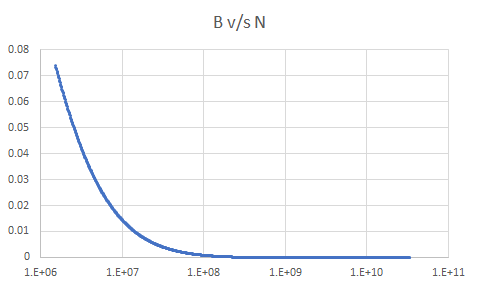
\includegraphics[width=0.6\linewidth]{B_vs_N.png}
  \caption{Plot of B v/s N}
  \label{fig:boat1}
\end{figure}

